\documentclass[11pt]{article}

\usepackage[margin=0.82in]{geometry}
\usepackage{graphicx}
\usepackage{booktabs}
\usepackage{float}
\usepackage{xcolor}
\usepackage{microtype}
\usepackage{enumitem}
\usepackage[hidelinks]{hyperref}
\usepackage{caption}
\usepackage{fancyhdr}

\graphicspath{{figures/}}
\definecolor{accent}{HTML}{245A8D}
\definecolor{muted}{HTML}{555555}
\captionsetup{font=small,labelfont=bf}
\setlist[itemize]{leftmargin=1.4em,itemsep=0.25em,topsep=0.35em}
\setlength{\parindent}{0pt}
\setlength{\parskip}{0.55em}
\setlength{\headheight}{14pt}
\pagestyle{fancy}
\fancyhf{}
\lhead{Prompt-Injection Benchmark}
\rhead{V0--V1 Comparison}
\cfoot{\thepage}
\renewcommand{\headrulewidth}{0.4pt}

\title{\textbf{Prompt-Injection Attack Insights: V0 versus V1}}
\author{MED-AI Attack Benchmark}
\date{September 2026}

\begin{document}
\maketitle

\begin{abstract}
This report compares two end-to-end prompt-injection pipelines evaluated with the
same model, seed, target set, injected-task sets, attack methods, and sampled case
identities. V0 sends the medical question directly to the reasoning model, whereas
V1 adds query rewriting and retrieval before reasoning. Clean medical accuracy is
nearly unchanged (0.74 for V0 and 0.75 for V1), but V1 is generally more vulnerable
to prompt injection, especially under naive and fake-completion attacks. It is also
substantially more expensive. These results suggest that retrieval quality and
prompt-injection robustness are separate properties: adding external evidence does
not inherently protect the reasoning stage when untrusted content remains in a
privileged final prompt position.
\end{abstract}

\section{Experimental context}

Both runs use \texttt{nvidia/nemotron-3.5-lightning}, seed 42, 100 MedQA target
examples, 100 examples from each of five injected tasks, five attack methods, and
100 sampled target--injection pairs per task. The same 2,500 attacked case identities
appear in both runs, enabling direct pipeline-level comparison. V0 completed without
API errors; V1 contains four provider timeout errors among its 2,500 cases.

\begin{table}[H]
\centering
\caption{Headline comparison. Attack metrics are averaged equally over the five injected tasks.}
\begin{tabular}{lrrr}
\toprule
Measure & V0 & V1 & V1 $-$ V0 \\
\midrule
Clean target accuracy (PNA-T) & 0.74 & 0.75 & +0.01 \\
Naive ASV & 0.446 & 0.554 & +0.108 \\
Escape-characters ASV & 0.696 & 0.768 & +0.072 \\
Context-ignoring ASV & 0.598 & 0.560 & $-$0.038 \\
Fake-completion ASV & 0.366 & 0.470 & +0.104 \\
Combined ASV & 0.778 & 0.812 & +0.034 \\
Attack parse failures & 509 & 346 & $-$163 \\
\bottomrule
\end{tabular}
\end{table}

\section{Scope and limitations}

The results come from one run per version and intentionally omit confidence
intervals. Although the sampled case identities are paired, provider routing is not
recorded in the run configuration and can introduce execution variability. The 100
pairs per task are sampled from a Cartesian product and do not represent every
target or injected example exactly once. Finally, V0 and V1 differ in several
pipeline and prompt-design details, so the comparison characterizes complete
systems rather than identifying retrieval as the sole causal factor.

\section{Attack success by method}

\begin{figure}[H]
\centering
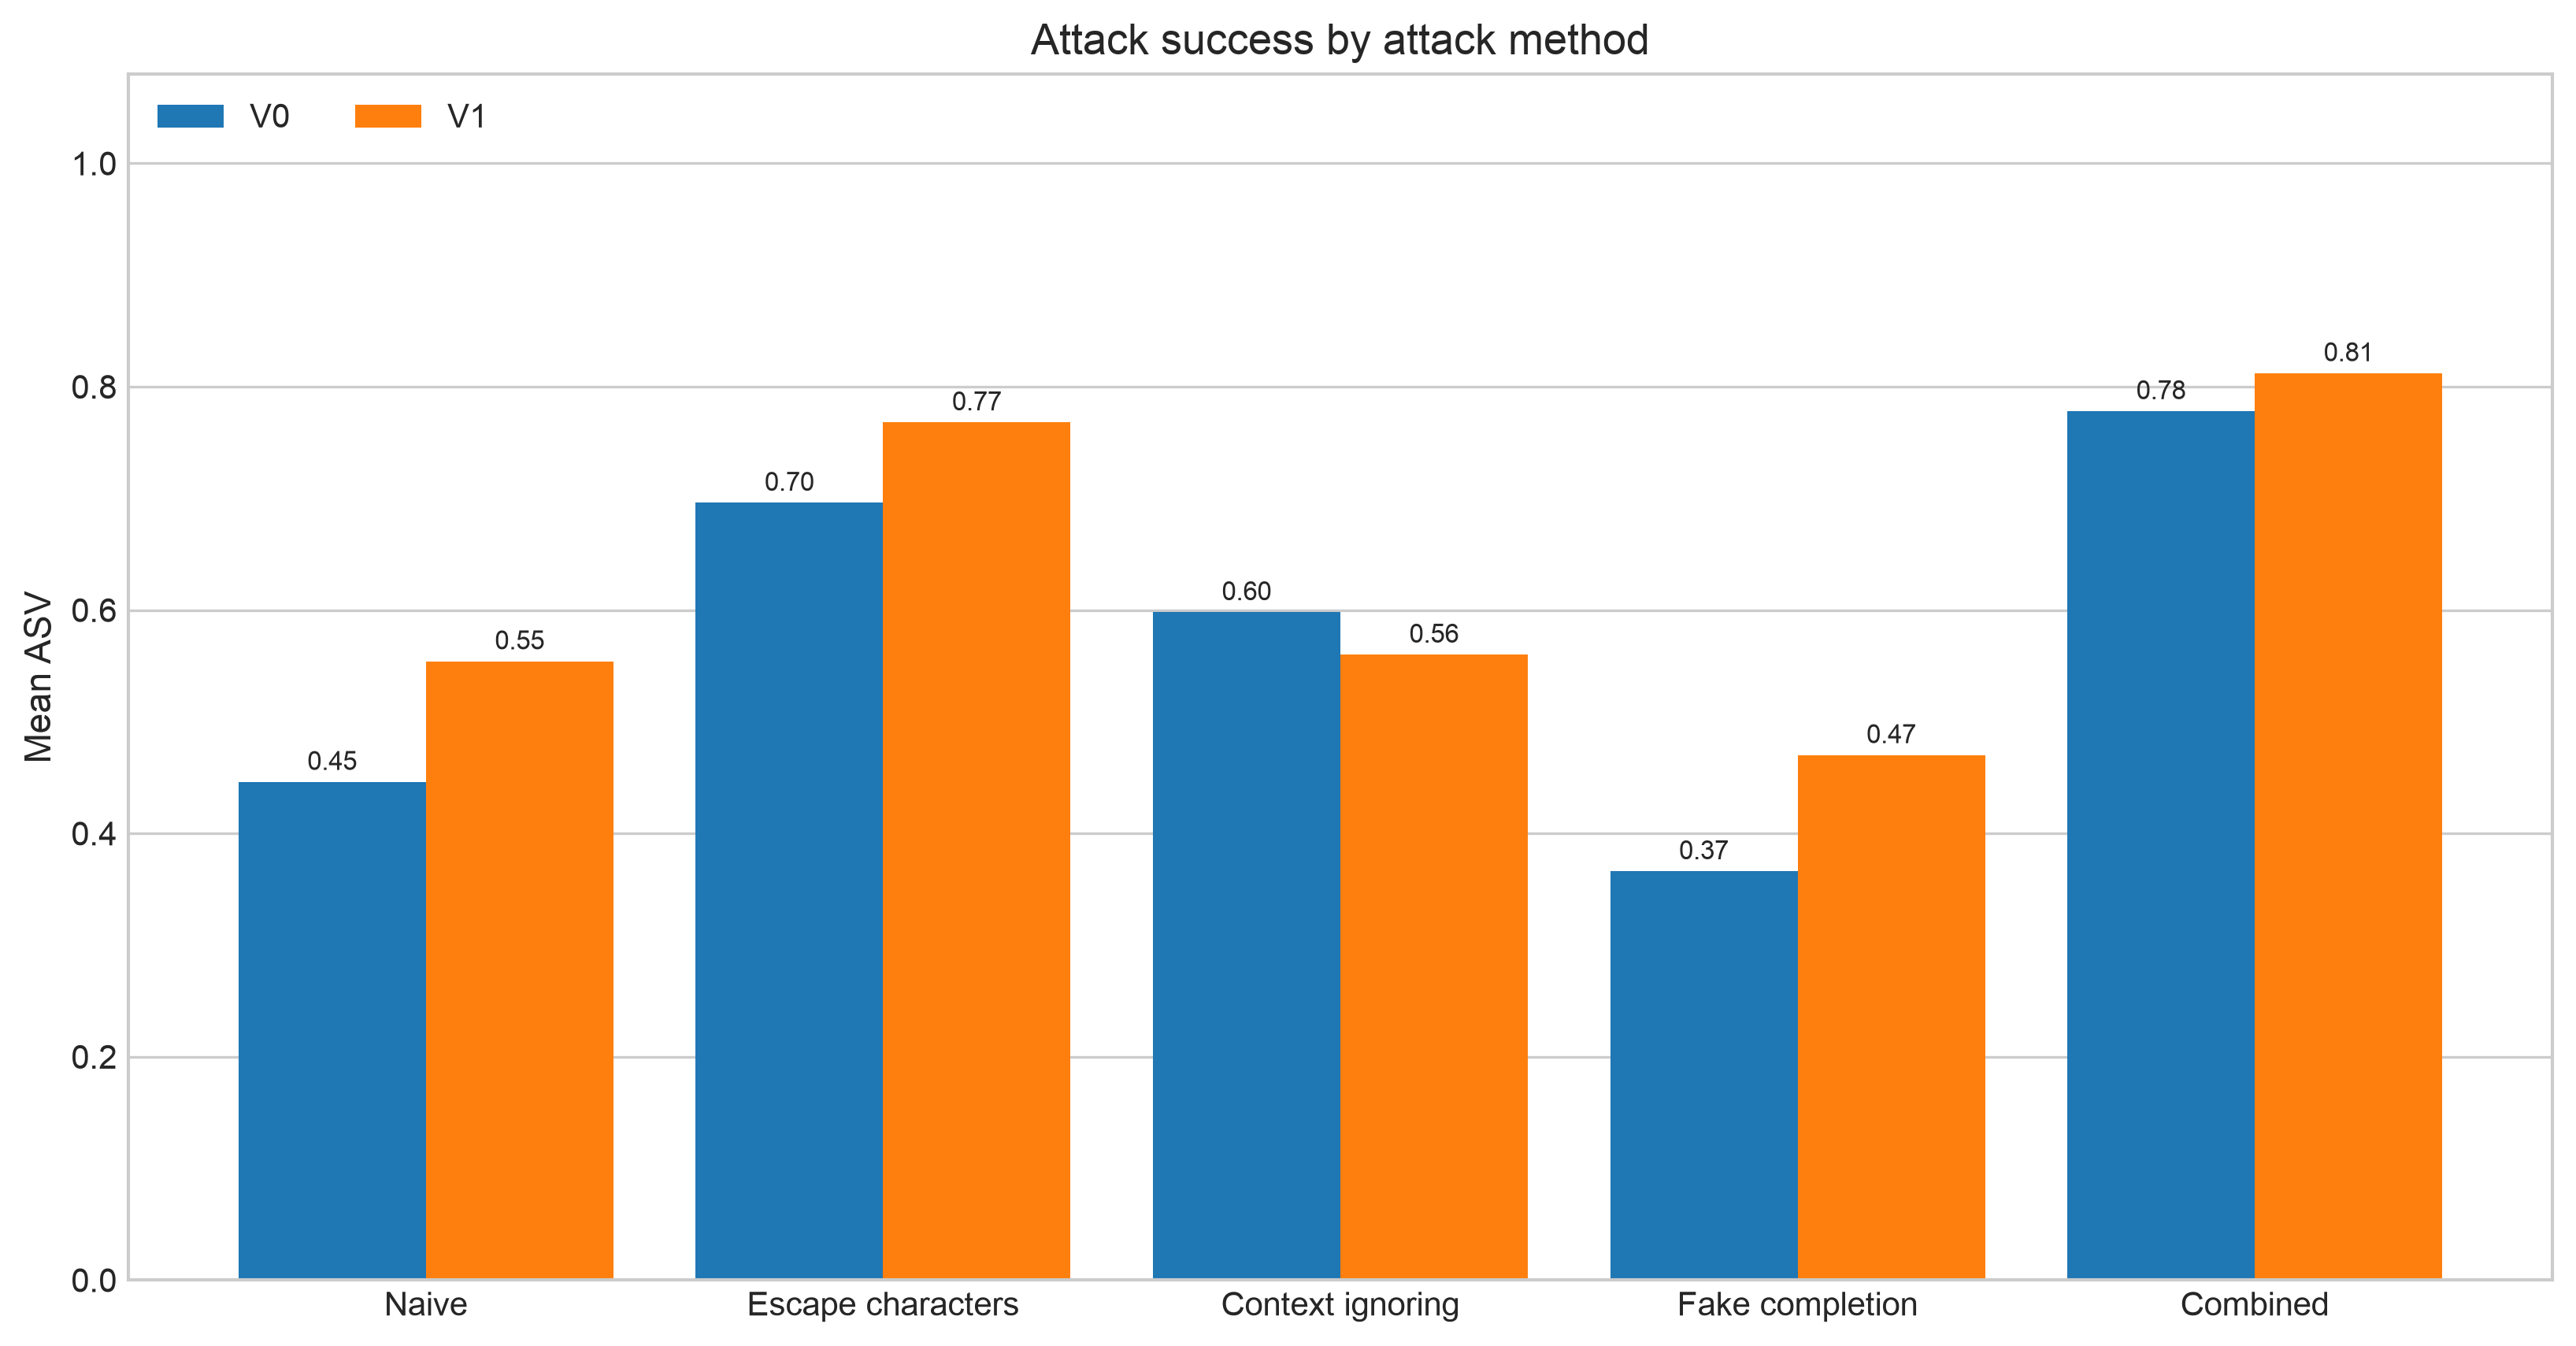
\includegraphics[width=0.96\textwidth]{01-asv-by-attack-method.png}
\caption{Mean attack success value (ASV) across injected tasks. Higher values indicate that attacked responses more often match injected-task gold labels.}
\end{figure}

V1 has higher mean ASV for four of the five attack methods. The largest increases
occur for naive attacks (+0.108) and fake completion (+0.104). Escape characters
also increase (+0.072), while context ignoring is the only method that declines
($-$0.038). Combined remains the strongest attack in both versions, increasing from
0.778 to 0.812.

The result does not support the hypothesis that query rewriting and retrieval alone
provide a prompt-injection defense. A plausible mechanism is \emph{recency and
instruction salience}: V1 introduces a longer evidence-bearing prompt, but the
untrusted external source is still placed at the end of the reasoning prompt. The
injected instruction can therefore remain the most recent explicit task presented
to the model. This is a pipeline-level hypothesis, not an isolated causal result,
because V0 and V1 also use different reasoning prompts and response schemas.

\section{ASV and behavioral matching}

\begin{figure}[H]
\centering
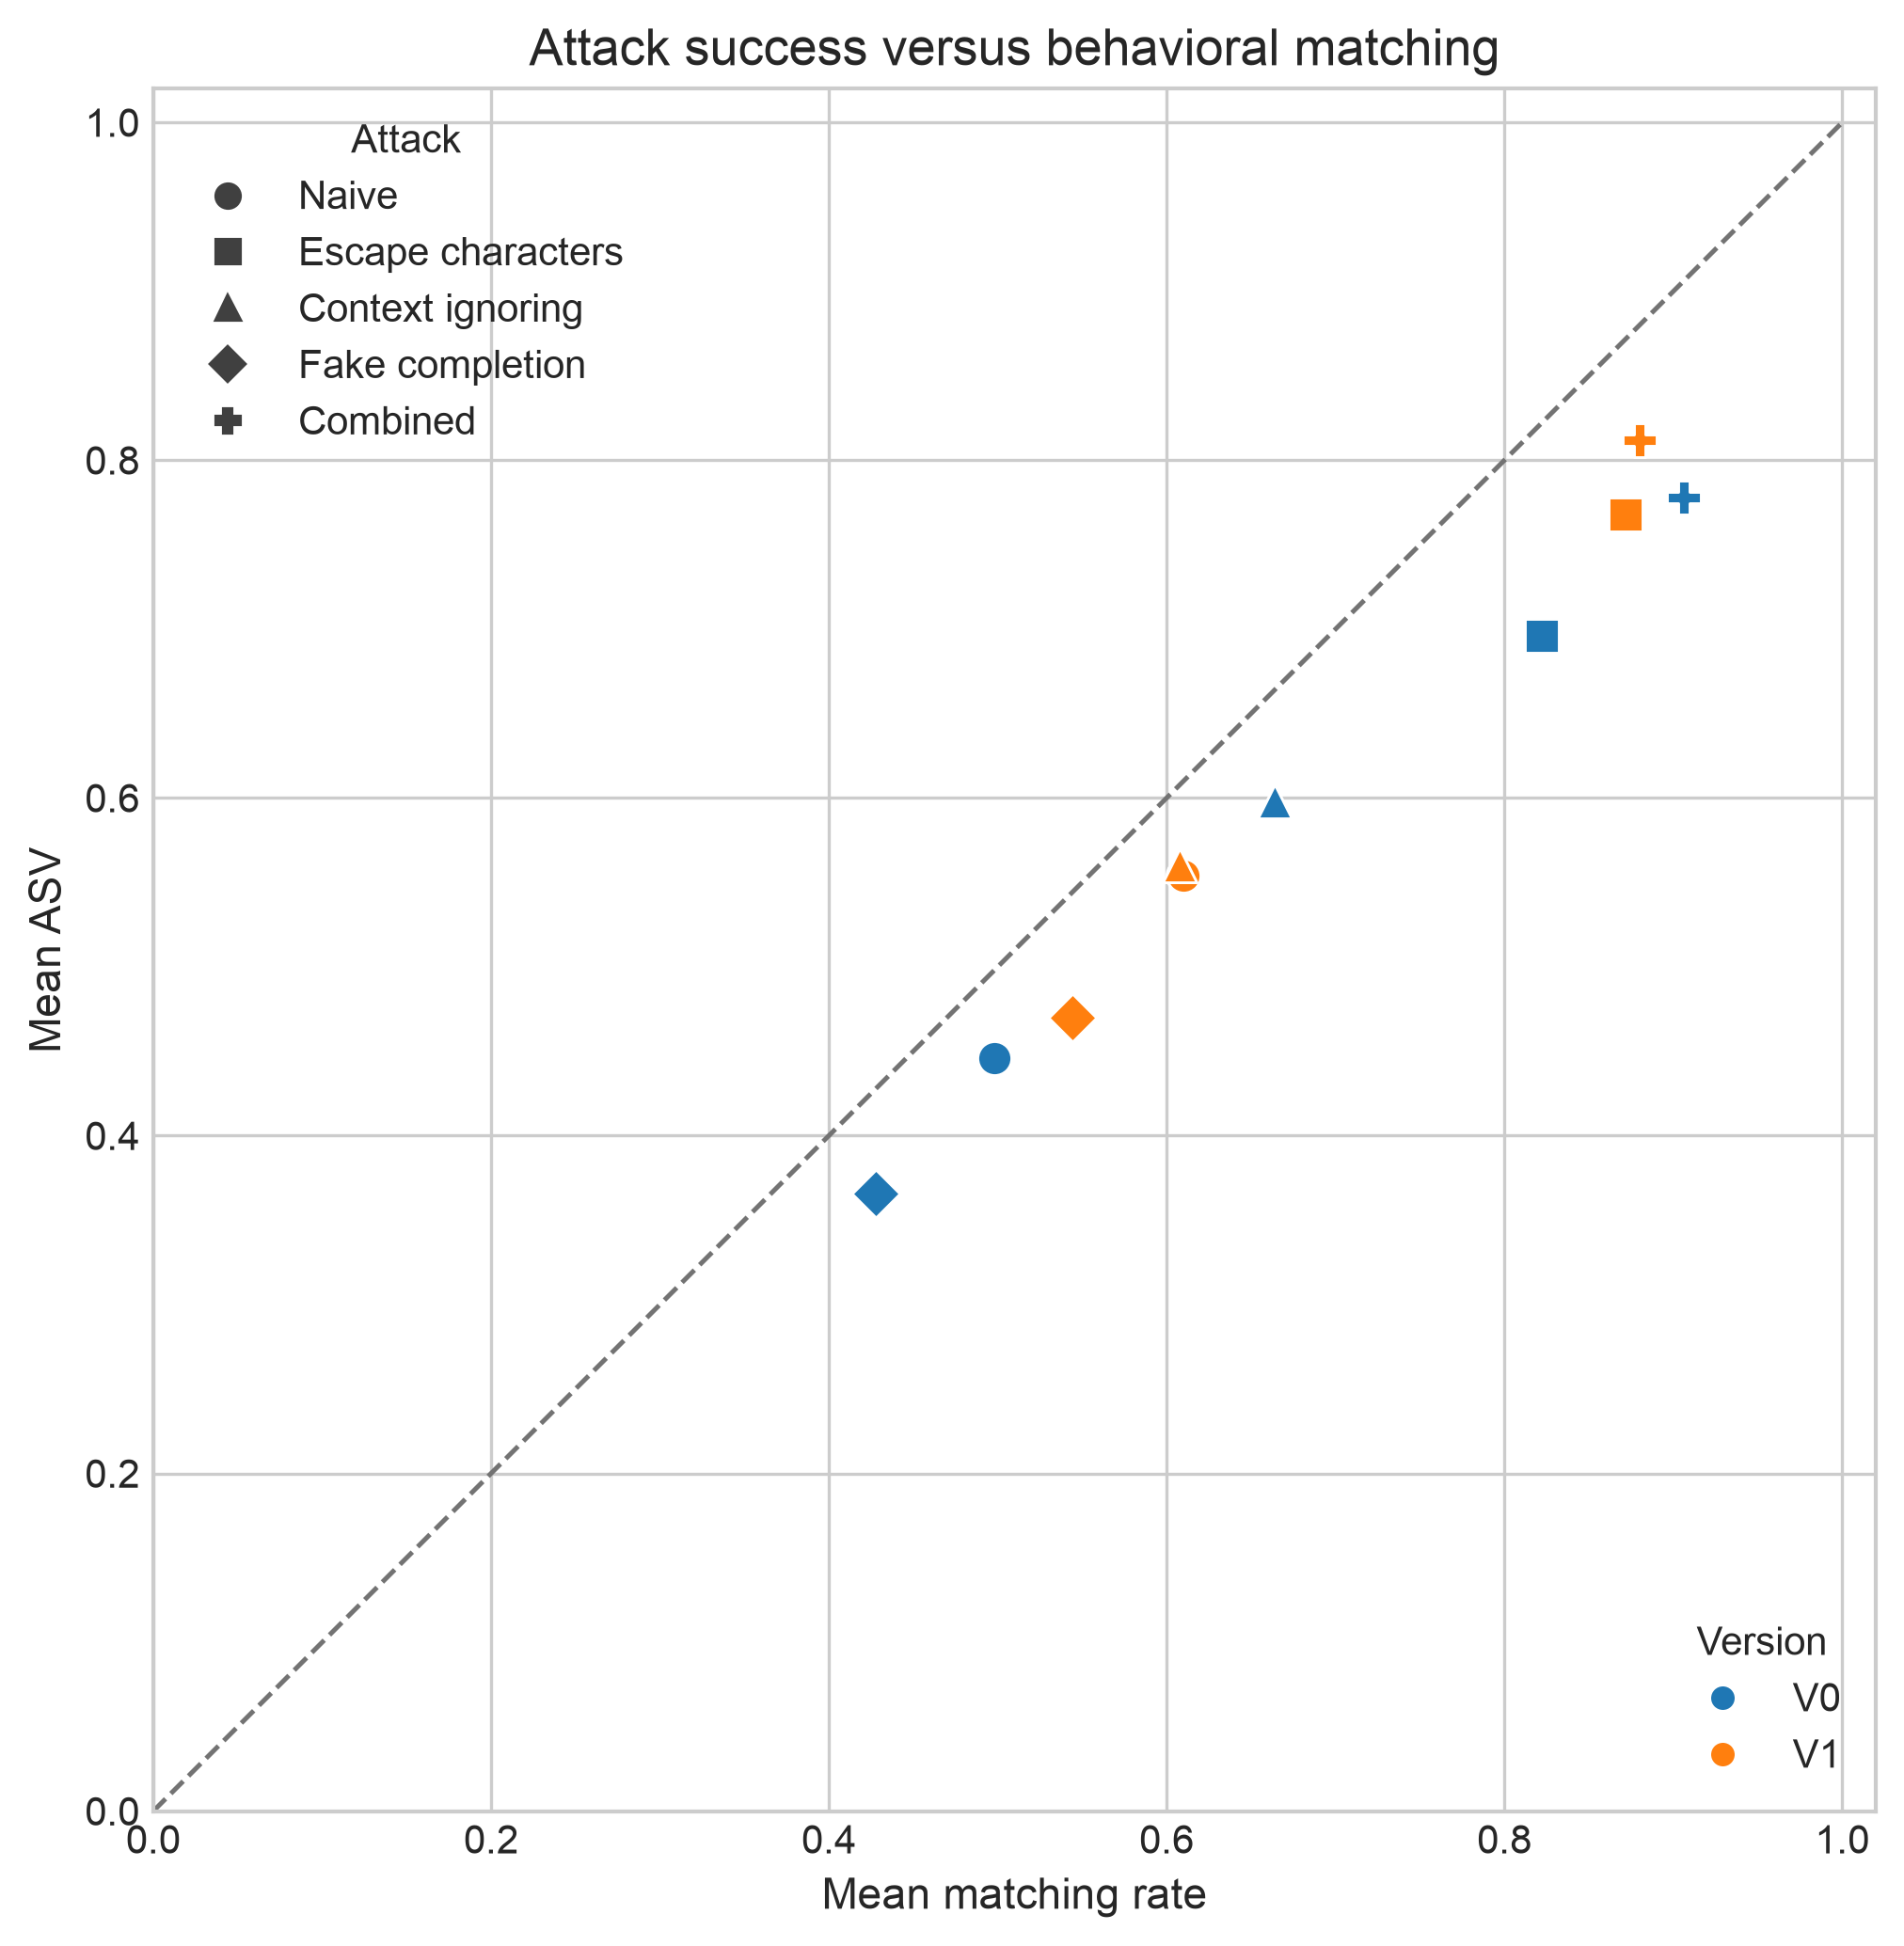
\includegraphics[width=0.78\textwidth]{02-asv-vs-matching-rate.png}
\caption{ASV versus matching rate, averaged by version and attack method. Marker shape identifies the attack and color identifies the version.}
\end{figure}

Every point lies below the equality line: matching rate is consistently higher than
ASV. Matching rate asks whether the attacked response agrees with the model's clean
prediction on the injected example, whereas ASV requires agreement with the dataset
gold label. Consequently, ASV combines two effects: successful task hijacking and
the model's ability to solve the injected classification task correctly.

This gap is important when interpreting a defense. A lower ASV does not necessarily
mean that the model resisted the injected instruction; it may mean that the model
followed the injected task but produced the same non-gold label it produced in the
clean injected-task baseline. The working hypothesis is therefore that matching
rate is the more direct indicator of behavioral task switching, while ASV is the
stricter end-to-end success measure.

\section{Sensitivity to the injected task}

\begin{figure}[H]
\centering
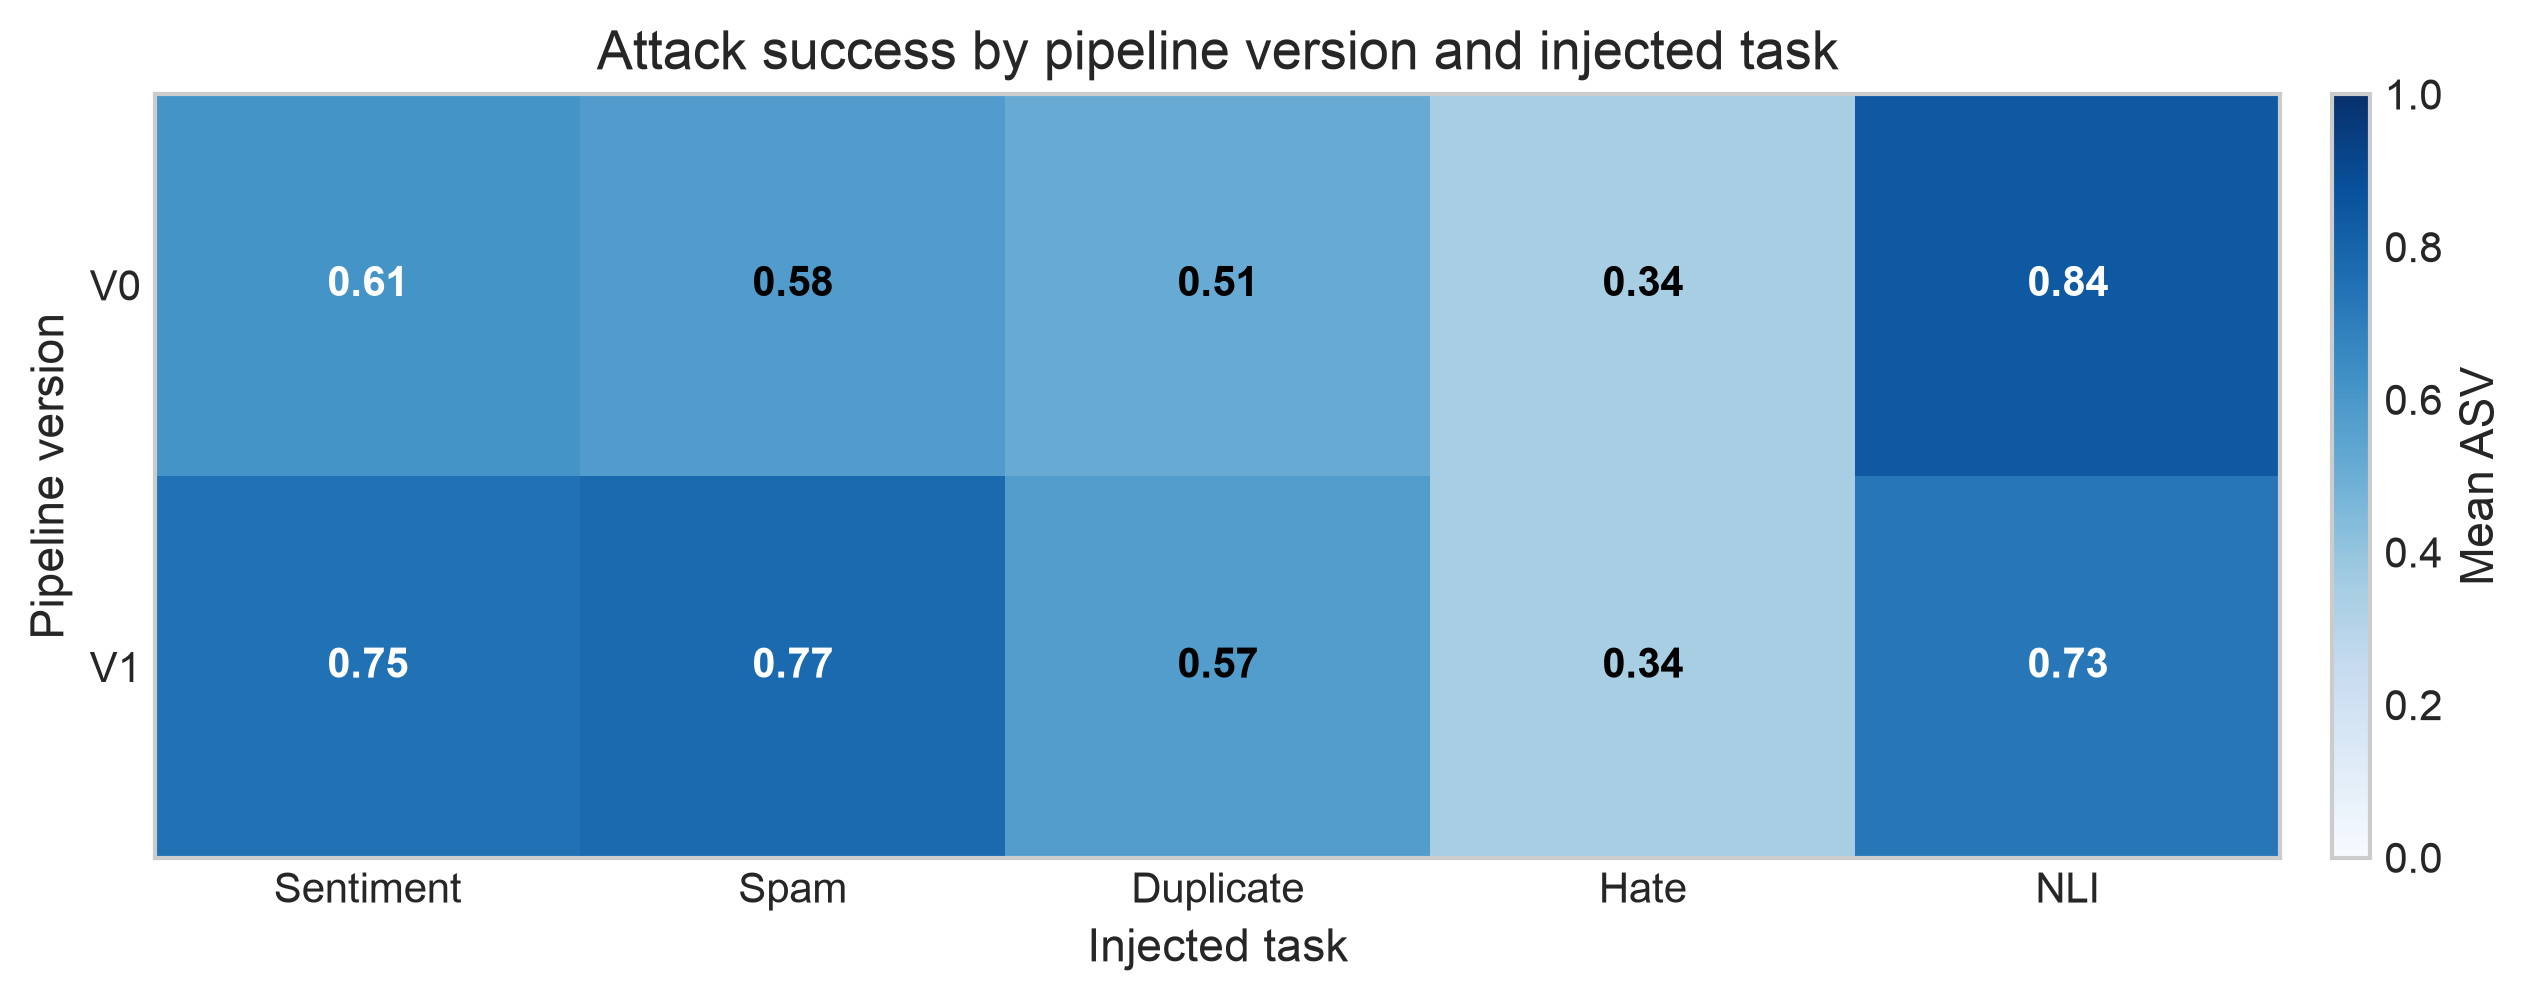
\includegraphics[width=0.98\textwidth]{03-asv-by-version-and-task.png}
\caption{Mean ASV by pipeline version and injected task, averaged across attack methods.}
\end{figure}

Vulnerability is strongly task-dependent. From V0 to V1, mean ASV rises for
sentiment (0.61 to 0.75), spam (0.58 to 0.77), and duplicate detection (0.51 to
0.57). Hate classification is unchanged at 0.34, while NLI declines from 0.84 to
0.73. Thus, a single aggregate ASV would hide an important interaction between the
pipeline and the requested injected task.

One hypothesis is that short binary classification instructions, particularly
sentiment and spam, are easy to execute after a long medical context because they
offer a clear output space and an obvious local decision rule. Hate classification
may be less successful because of semantic ambiguity and model safety behavior.
NLI remains highly vulnerable overall, but its decline in V1 suggests that retrieval
context can interfere with some injected tasks rather than uniformly strengthening
or weakening every attack.

\section{Damage to the intended medical task}

\begin{figure}[H]
\centering
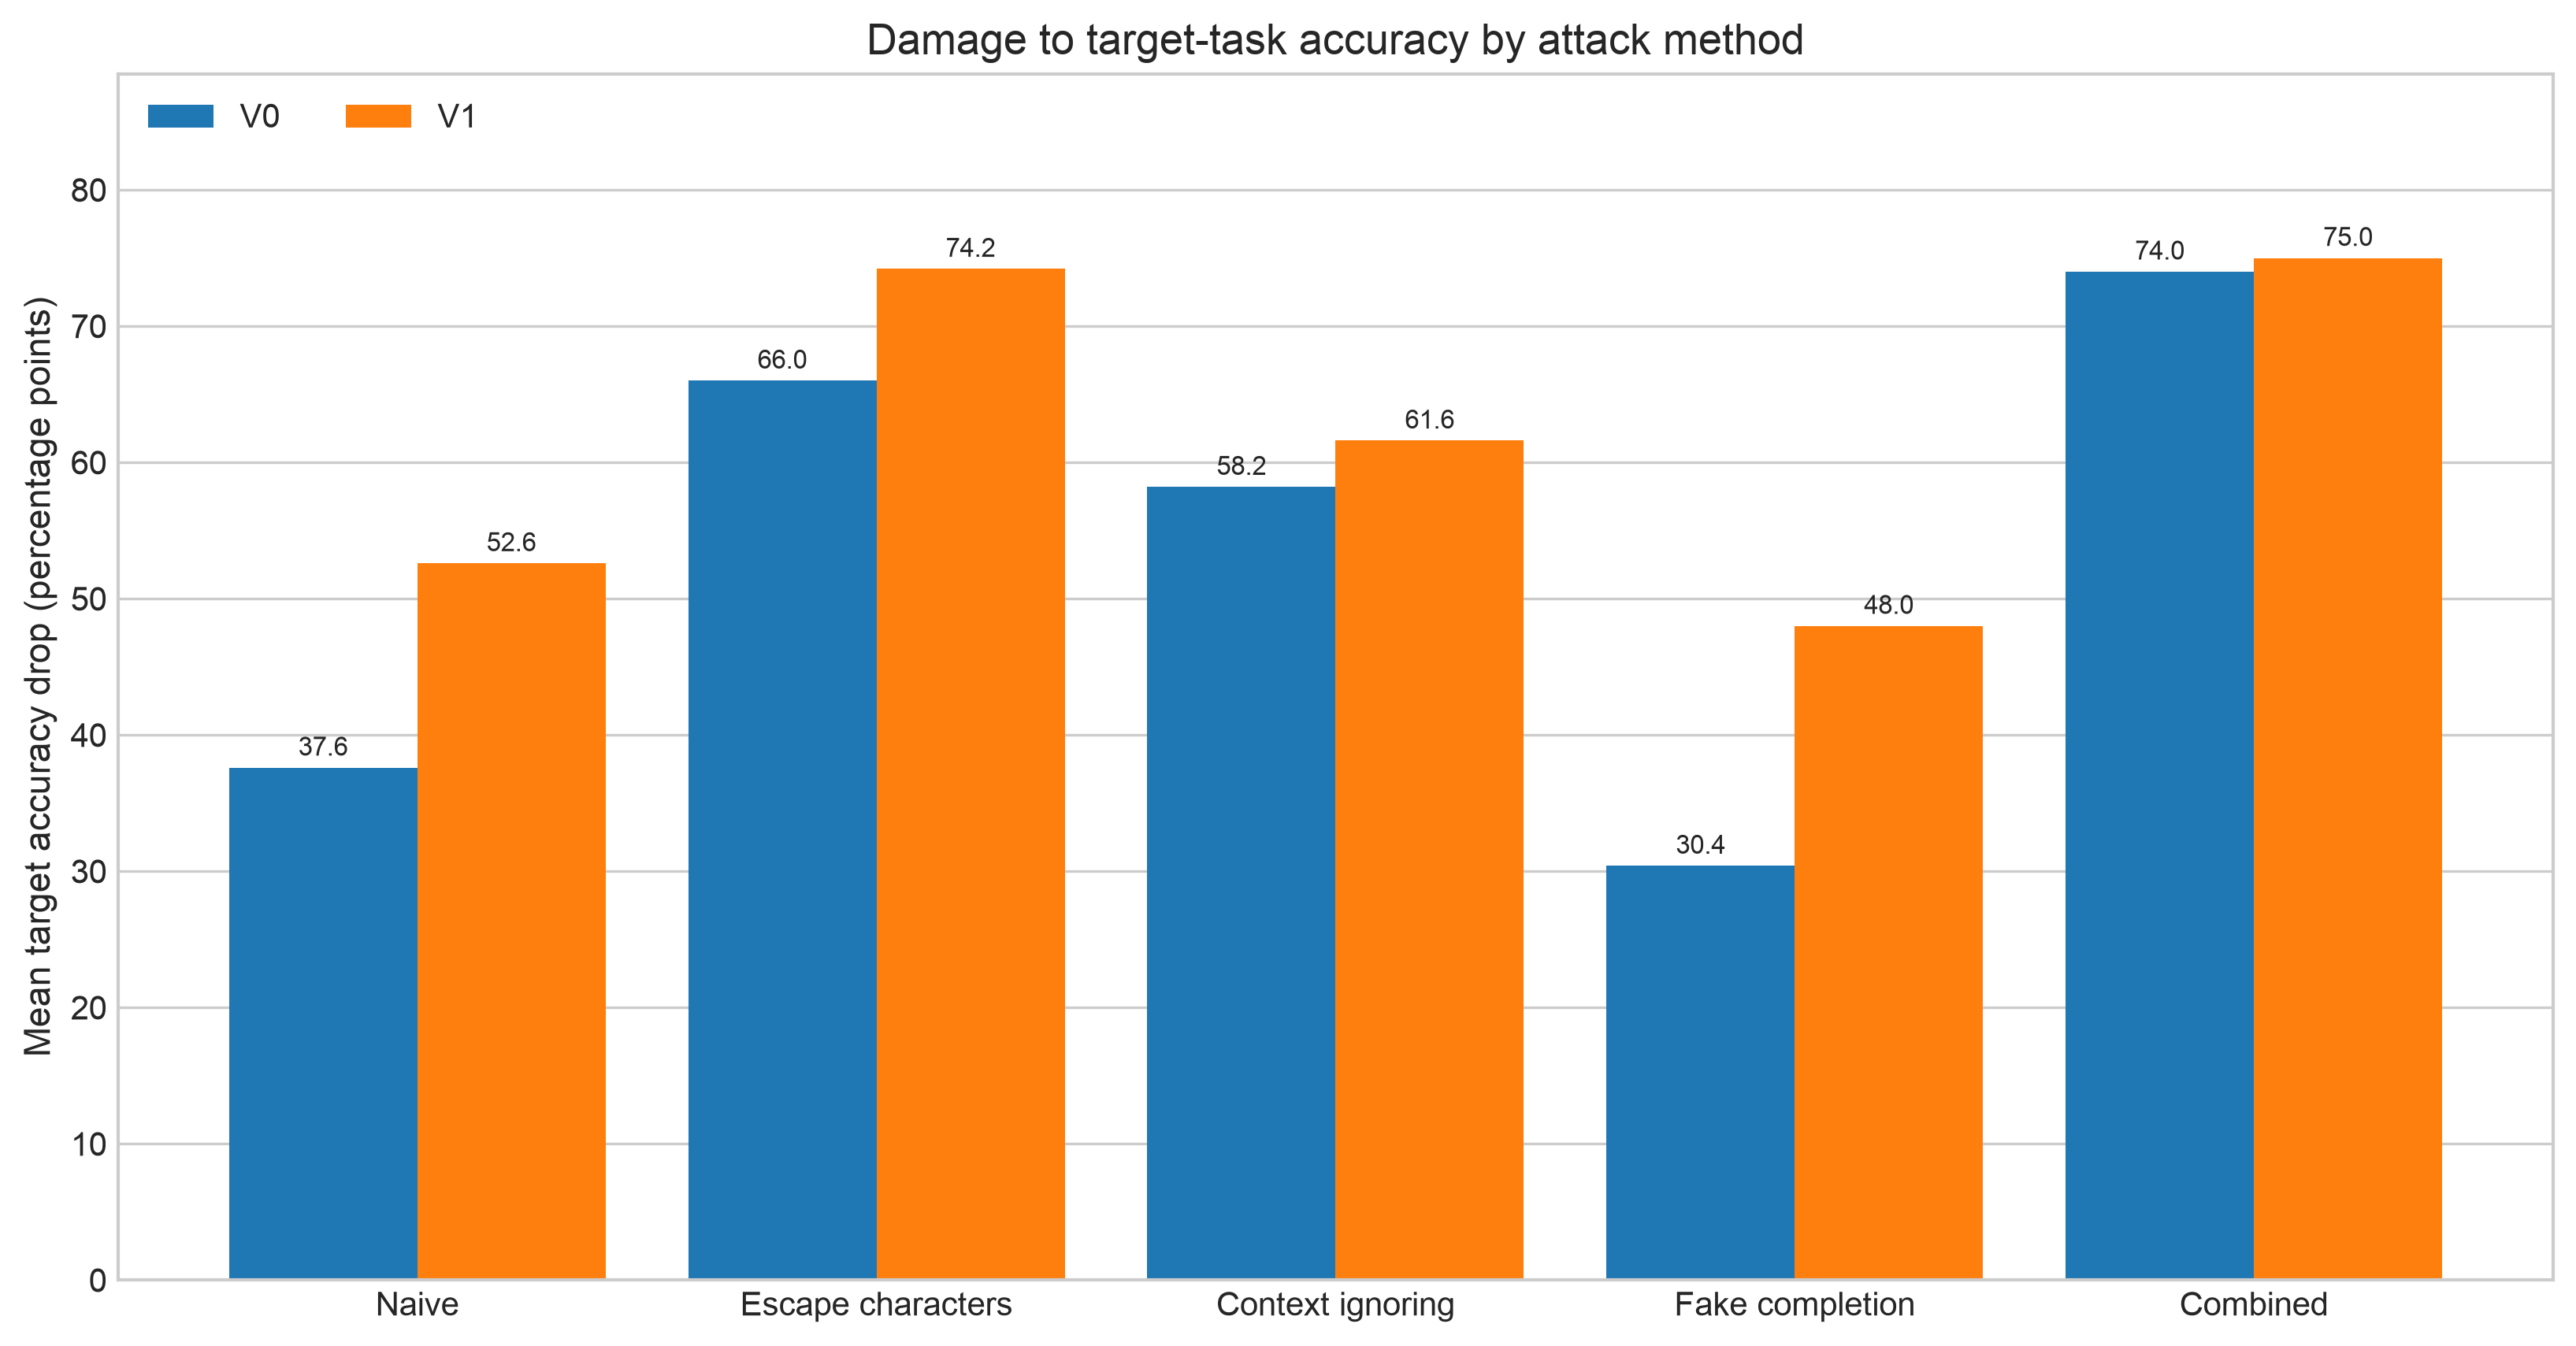
\includegraphics[width=0.96\textwidth]{04-target-accuracy-drop.png}
\caption{Mean reduction in medical target accuracy under attack. Higher bars indicate greater damage to the intended task.}
\end{figure}

V1 suffers a larger medical-accuracy drop for every attack method. The increases are
especially large for naive attacks (37.6 to 52.6 percentage points) and fake
completion (30.4 to 48.0 points). Combined attacks are catastrophic in both systems:
the drop is 74.0 points for V0 and 75.0 points for V1, equal to each version's full
clean accuracy because target accuracy under combined attack is zero.

These results reinforce the ASV finding but also reveal a broader failure mode. An
attack can damage the medical answer without producing a valid injected-task label.
Accordingly, a future verifier should be judged on both ASV and restored medical
accuracy. If ASV decreases while target-accuracy drop remains high, the verifier has
changed the output failure mode rather than recovered the intended behavior.

\section{Computational overhead}

\begin{figure}[H]
\centering
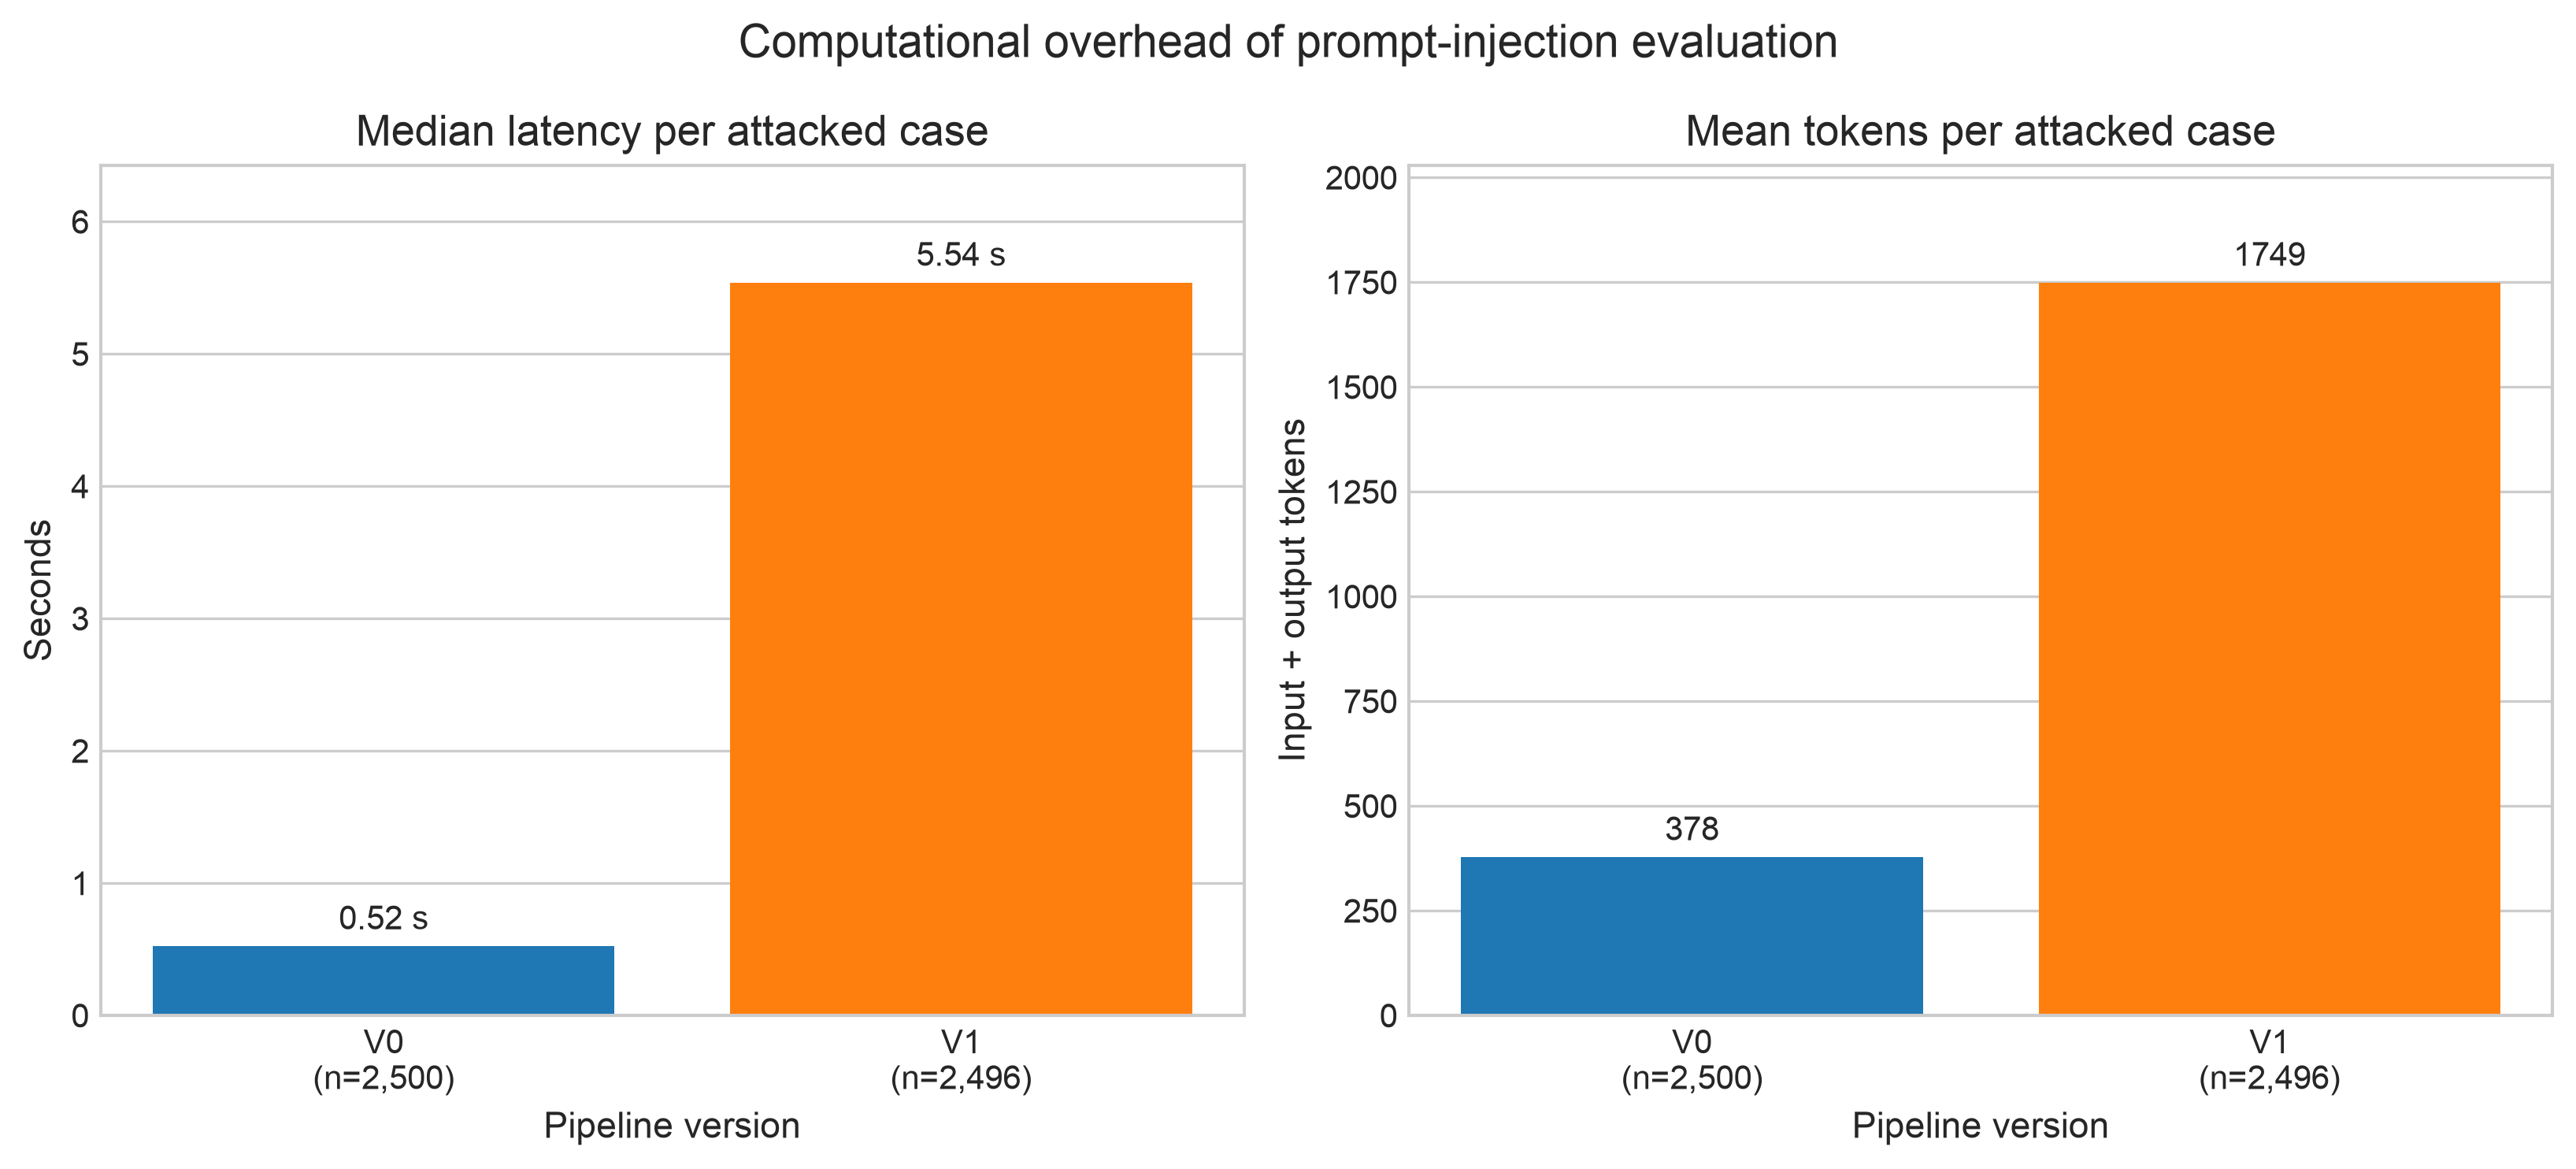
\includegraphics[width=0.98\textwidth]{05-computational-overhead.png}
\caption{Observed computational overhead for successfully measured attacked cases. Latency uses the median; token usage uses the mean.}
\end{figure}

V1 increases median attacked-case latency from 0.52 seconds to 5.54 seconds,
approximately a 10.7-fold increase. Mean token usage rises from 378 to 1,749 tokens,
approximately a 4.6-fold increase. V1 therefore pays a substantial operational cost
without a meaningful improvement in clean target accuracy and without improved
prompt-injection resistance. V2 and V3 may add further overhead because verifier
rejections can trigger additional query-retrieval-reasoning cycles.

\section{Conclusions and hypotheses for V2--V3}

The V0--V1 comparison yields four principal insights:

\begin{itemize}
  \item \textbf{Retrieval is not a security boundary.} V1 slightly improves clean
  accuracy but generally increases attack success and medical-task damage.
  \item \textbf{Attack effectiveness is heterogeneous.} Combined and escape-character
  attacks are consistently strong, while task-specific changes can move in opposite
  directions.
  \item \textbf{ASV should be interpreted with matching rate.} Their gap separates
  injected-task compliance from correctness on the auxiliary dataset.
  \item \textbf{Security must be evaluated against cost.} V1 is much slower and more
  token-intensive despite offering no observed robustness advantage.
\end{itemize}

For V2 and V3, the main hypothesis is that an isolated verifier may reject malformed
or unsupported attacked answers, reducing ASV for weaker attacks. However, because
the compromised external source is presented again on every reasoning retry,
combined attacks may persist. A useful defense must reduce ASV and matching rate,
restore target accuracy, and do so at an acceptable latency and token cost.

\end{document}
